\documentclass[11pt,a3paper,landscape]{article}
\usepackage[utf8]{inputenc}
\usepackage[T1]{fontenc}
\usepackage[paperwidth=42cm,paperheight=29.7cm,margin=0.8cm]{geometry}
\usepackage{tikz}
\usepackage{graphicx}
\usetikzlibrary{arrows.meta,positioning,fit,backgrounds,calc}

\definecolor{pastelRuntime}{RGB}{220,234,252}
\definecolor{pastelApi}{RGB}{226,245,230}
\definecolor{pastelServices}{RGB}{255,239,219}
\definecolor{pastelSchemas}{RGB}{236,230,252}
\definecolor{pastelModels}{RGB}{255,226,235}
\definecolor{pastelExceptions}{RGB}{255,243,214}

\begin{document}
\pagestyle{empty}

\begin{center}
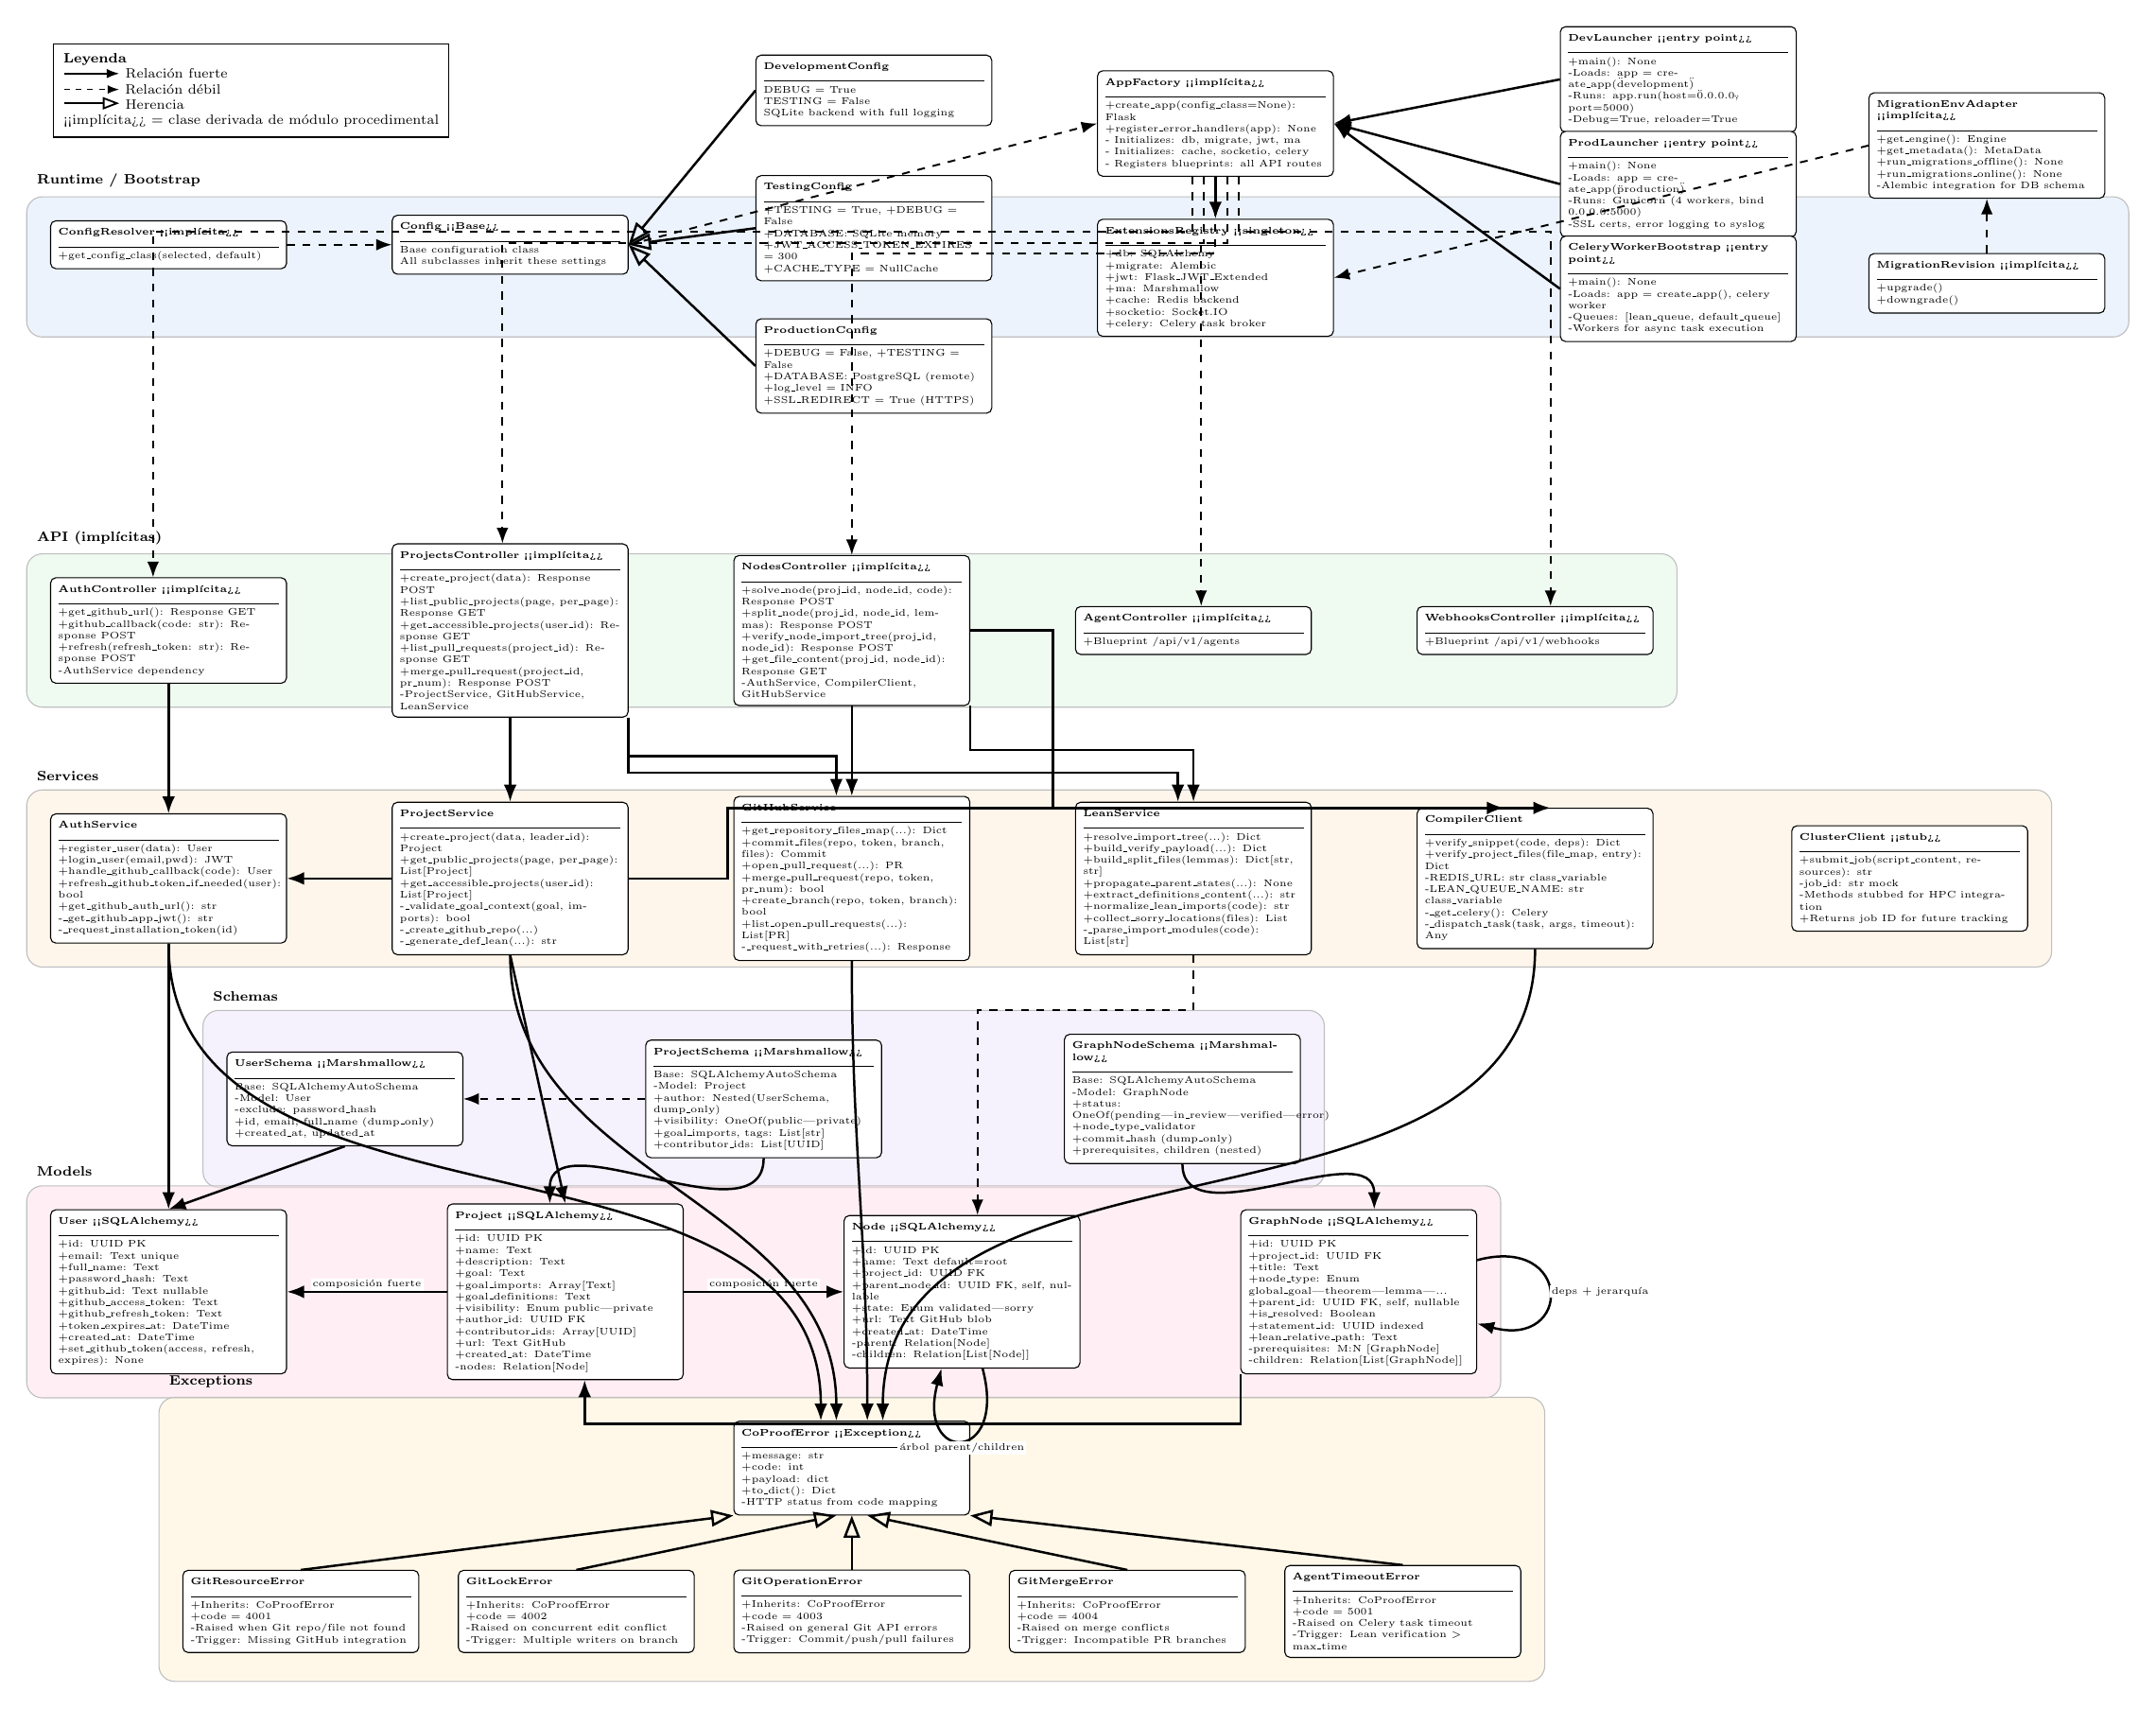
\begin{tikzpicture}[
  scale=0.74,
  transform shape,
  x=1cm,
  y=1cm,
  classbox/.style={
    draw,
    rounded corners=2pt,
    align=left,
    font=\tiny,
    text width=4.0cm,
    inner sep=4pt,
    fill=white
  },
  sectionbox/.style={draw=black!25, line width=0.4pt, rounded corners=6pt, inner sep=9pt, fill opacity=0.55},
  strong/.style={-{Latex[length=2.3mm]}, line width=0.9pt},
  weak/.style={-{Latex[length=2.1mm]}, line width=0.7pt, dashed},
  inherit/.style={-{Triangle[open,length=3mm,width=2.2mm]}, line width=0.9pt},
  rel/.style={font=\tiny, fill=white, inner sep=1pt}
]

% =========================
% Runtime / Bootstrap
% =========================
\node[classbox] (configResolver) at (0,12) {
\textbf{ConfigResolver <<implícita>>}\\
\rule{\linewidth}{0.2pt}\\
+get\_config\_class(selected, default)
};

\node[classbox] (config) at (6.2,12) {
\textbf{Config <<Base>>}\\
\rule{\linewidth}{0.2pt}\\
Base configuration class\\
All subclasses inherit these settings
};

\node[classbox] (devConfig) at (12.8,14.8) {
\textbf{DevelopmentConfig}\\
\rule{\linewidth}{0.2pt}\\
DEBUG = True\\
TESTING = False\\
SQLite backend with full logging
};

\node[classbox] (testConfig) at (12.8,12.3) {
\textbf{TestingConfig}\\
\rule{\linewidth}{0.2pt}\\
+TESTING = True, +DEBUG = False\\
+DATABASE: SQLite memory\\
+JWT\_ACCESS\_TOKEN\_EXPIRES = 300\\
+CACHE\_TYPE = NullCache
};

\node[classbox] (prodConfig) at (12.8,9.8) {
\textbf{ProductionConfig}\\
\rule{\linewidth}{0.2pt}\\
+DEBUG = False, +TESTING = False\\
+DATABASE: PostgreSQL (remote)\\
+log\_level = INFO\\
+SSL\_REDIRECT = True (HTTPS)
};

\node[classbox] (extensions) at (19,11.4) {
\textbf{ExtensionsRegistry <<singleton>>}\\
\rule{\linewidth}{0.2pt}\\
+db: SQLAlchemy\\
+migrate: Alembic\\
+jwt: Flask\_JWT\_Extended\\
+ma: Marshmallow\\
+cache: Redis backend\\
+socketio: Socket.IO\\
+celery: Celery task broker
};

\node[classbox] (appFactory) at (19,14.2) {
\textbf{AppFactory <<implícita>>}\\
\rule{\linewidth}{0.2pt}\\
+create\_app(config\_class=None): Flask\\
+register\_error\_handlers(app): None\\
- Initializes: db, migrate, jwt, ma\\
- Initializes: cache, socketio, celery\\
- Registers blueprints: all API routes
};

\node[classbox] (devLauncher) at (27.4,15.0) {
\textbf{DevLauncher <<entry point>>}\\
\rule{\linewidth}{0.2pt}\\
+main(): None\\
-Loads: app = create\_app(\"development\")\\
-Runs: app.run(host=\"0.0.0.0\", port=5000)\\
-Debug=True, reloader=True
};

\node[classbox] (prodLauncher) at (27.4,13.1) {
\textbf{ProdLauncher <<entry point>>}\\
\rule{\linewidth}{0.2pt}\\
+main(): None\\
-Loads: app = create\_app(\"production\")\\
-Runs: Gunicorn (4 workers, bind 0.0.0.0:5000)\\
-SSL certs, error logging to syslog
};

\node[classbox] (celeryBoot) at (27.4,11.2) {
\textbf{CeleryWorkerBootstrap <<entry point>>}\\
\rule{\linewidth}{0.2pt}\\
+main(): None\\
-Loads: app = create\_app(), celery worker\\
-Queues: [lean\_queue, default\_queue]\\
-Workers for async task execution
};

\node[classbox] (migrationEnv) at (33.0,13.8) {
\textbf{MigrationEnvAdapter <<implícita>>}\\
\rule{\linewidth}{0.2pt}\\
+get\_engine(): Engine\\
+get\_metadata(): MetaData\\
+run\_migrations\_offline(): None\\
+run\_migrations\_online(): None\\
-Alembic integration for DB schema
};

\node[classbox] (migrationRev) at (33.0,11.3) {
\textbf{MigrationRevision <<implícita>>}\\
\rule{\linewidth}{0.2pt}\\
+upgrade()\\
+downgrade()
};

% =========================
% API Layer (procedural -> implicit classes)
% =========================
\node[classbox] (authCtrl) at (0,5) {
\textbf{AuthController <<implícita>>}\\
\rule{\linewidth}{0.2pt}\\
+get\_github\_url(): Response {GET}\\
+github\_callback(code: str): Response {POST}\\
+refresh(refresh\_token: str): Response {POST}\\
-AuthService dependency
};

\node[classbox] (projectsCtrl) at (6.2,5) {
\textbf{ProjectsController <<implícita>>}\\
\rule{\linewidth}{0.2pt}\\
+create\_project(data): Response {POST}\\
+list\_public\_projects(page, per\_page): Response {GET}\\
+get\_accessible\_projects(user\_id): Response {GET}\\
+list\_pull\_requests(project\_id): Response {GET}\\
+merge\_pull\_request(project\_id, pr\_num): Response {POST}\\
-ProjectService, GitHubService, LeanService
};

\node[classbox] (nodesCtrl) at (12.4,5) {
\textbf{NodesController <<implícita>>}\\
\rule{\linewidth}{0.2pt}\\
+solve\_node(proj\_id, node\_id, code): Response {POST}\\
+split\_node(proj\_id, node\_id, lemmas): Response {POST}\\
+verify\_node\_import\_tree(proj\_id, node\_id): Response {POST}\\
+get\_file\_content(proj\_id, node\_id): Response {GET}\\
-AuthService, CompilerClient, GitHubService
};

\node[classbox] (agentCtrl) at (18.6,5) {
\textbf{AgentController <<implícita>>}\\
\rule{\linewidth}{0.2pt}\\
+Blueprint /api/v1/agents
};

\node[classbox] (webhookCtrl) at (24.8,5) {
\textbf{WebhooksController <<implícita>>}\\
\rule{\linewidth}{0.2pt}\\
+Blueprint /api/v1/webhooks
};

% =========================
% Services
% =========================
\node[classbox] (authService) at (0,0.5) {
\textbf{AuthService}\\\rule{\linewidth}{0.2pt}\\
+register\_user(data): User\\
+login\_user(email,pwd): JWT\\
+handle\_github\_callback(code): User\\
+refresh\_github\_token\_if\_needed(user): bool\\
+get\_github\_auth\_url(): str\\
-\_get\_github\_app\_jwt(): str\\
-\_request\_installation\_token(id)
};

\node[classbox] (projectService) at (6.2,0.5) {
\textbf{ProjectService}\\
\rule{\linewidth}{0.2pt}\\
+create\_project(data, leader\_id): Project\\
+get\_public\_projects(page, per\_page): List[Project]\\
+get\_accessible\_projects(user\_id): List[Project]\\
-\_validate\_goal\_context(goal, imports): bool\\
-\_create\_github\_repo(...)\\
-\_generate\_def\_lean(...): str
};

\node[classbox] (githubService) at (12.4,0.5) {
\textbf{GitHubService}\\
\rule{\linewidth}{0.2pt}\\
+get\_repository\_files\_map(...): Dict\\
+commit\_files(repo, token, branch, files): Commit\\
+open\_pull\_request(...): PR\\
+merge\_pull\_request(repo, token, pr\_num): bool\\
+create\_branch(repo, token, branch): bool\\
+list\_open\_pull\_requests(...): List[PR]\\
-\_request\_with\_retries(...): Response
};

\node[classbox] (leanService) at (18.6,0.5) {
\textbf{LeanService}\\
\rule{\linewidth}{0.2pt}\\
+resolve\_import\_tree(...): Dict\\
+build\_verify\_payload(...): Dict\\
+build\_split\_files(lemmas): Dict[str, str]\\
+propagate\_parent\_states(...): None\\
+extract\_definitions\_content(...): str\\
+normalize\_lean\_imports(code): str\\
+collect\_sorry\_locations(files): List\\
-\_parse\_import\_modules(code): List[str]
};

\node[classbox] (compilerClient) at (24.8,0.5) {
\textbf{CompilerClient}\\
\rule{\linewidth}{0.2pt}\\
+verify\_snippet(code, deps): Dict\\
+verify\_project\_files(file\_map, entry): Dict\\
-REDIS\_URL: str {class\_variable}\\
-LEAN\_QUEUE\_NAME: str {class\_variable}\\
-\_get\_celery(): Celery\\
-\_dispatch\_task(task, args, timeout): Any
};

\node[classbox] (clusterClient) at (31.6,0.5) {
\textbf{ClusterClient <<stub>>}\\
\rule{\linewidth}{0.2pt}\\
+submit\_job(script\_content, resources): str\\
-job\_id: str {mock}\\
-Methods stubbed for HPC integration\\
+Returns job ID for future tracking
};

% =========================
% Schemas
% =========================
\node[classbox] (userSchema) at (3.2,-3.5) {
\textbf{UserSchema <<Marshmallow>>}\\
\rule{\linewidth}{0.2pt}\\
Base: SQLAlchemyAutoSchema\\
-Model: User\\
-exclude: {password\_hash}\\
+id, email, full\_name (dump\_only)\\
+created\_at, updated\_at
};

\node[classbox] (projectSchema) at (10.8,-3.5) {
\textbf{ProjectSchema <<Marshmallow>>}\\
\rule{\linewidth}{0.2pt}\\
Base: SQLAlchemyAutoSchema\\
-Model: Project\\
+author: Nested(UserSchema, dump\_only)\\
+visibility: OneOf(public|private)\\
+goal\_imports, tags: List[str]\\
+contributor\_ids: List[UUID]
};

\node[classbox] (graphNodeSchema) at (18.4,-3.5) {
\textbf{GraphNodeSchema <<Marshmallow>>}\\
\rule{\linewidth}{0.2pt}\\
Base: SQLAlchemyAutoSchema\\
-Model: GraphNode\\
+status: OneOf(pending|in\_review|verified|error)\\
+node\_type\_validator\\
+commit\_hash (dump\_only)\\
+prerequisites, children (nested)
};

% =========================
% Models
% =========================
\node[classbox] (userModel) at (0,-7) {
\textbf{User <<SQLAlchemy>>}\\
\rule{\linewidth}{0.2pt}\\
+id: UUID {PK}\\
+email: Text {unique}\\
+full\_name: Text\\
+password\_hash: Text\\
+github\_id: Text {nullable}\\
+github\_access\_token: Text\\
+github\_refresh\_token: Text\\
+token\_expires\_at: DateTime\\
+created\_at: DateTime\\
+set\_github\_token(access, refresh, expires): None
};

\node[classbox] (projectModel) at (7.2,-7) {
\textbf{Project <<SQLAlchemy>>}\\
\rule{\linewidth}{0.2pt}\\
+id: UUID {PK}\\
+name: Text\\
+description: Text\\
+goal: Text\\
+goal\_imports: Array[Text]\\
+goal\_definitions: Text\\
+visibility: Enum {public|private}\\
+author\_id: UUID {FK}\\
+contributor\_ids: Array[UUID]\\
+url: Text {GitHub}\\
+created\_at: DateTime\\
-nodes: Relation[Node]
};

\node[classbox] (nodeModel) at (14.4,-7) {
\textbf{Node <<SQLAlchemy>>}\\
\rule{\linewidth}{0.2pt}\\
+id: UUID {PK}\\
+name: Text {default=root}\\
+project\_id: UUID {FK}\\
+parent\_node\_id: UUID {FK, self, nullable}\\
+state: Enum {validated|sorry}\\
+url: Text {GitHub blob}\\
+created\_at: DateTime\\
-parent: Relation[Node]\\
-children: Relation[List[Node]]
};

\node[classbox] (graphNodeModel) at (21.6,-7) {
\textbf{GraphNode <<SQLAlchemy>>}\\
\rule{\linewidth}{0.2pt}\\
+id: UUID {PK}\\
+project\_id: UUID {FK}\\
+title: Text\\
+node\_type: Enum {global\_goal|theorem|lemma|...}\\
+parent\_id: UUID {FK, self, nullable}\\
+is\_resolved: Boolean\\
+statement\_id: UUID {indexed}\\
+lean\_relative\_path: Text\\
-prerequisites: M:N [GraphNode]\\
-children: Relation[List[GraphNode]]
};

% =========================
% Exceptions
% =========================
\node[classbox] (coProofErr) at (12.4,-10.2) {
\textbf{CoProofError <<Exception>>}\\
\rule{\linewidth}{0.2pt}\\
+message: str\\
+code: int\\
+payload: dict\\
+to\_dict(): Dict\\
-HTTP status from code mapping
};

\node[classbox] (gitResourceErr) at (2.4,-12.8) {
\textbf{GitResourceError}\\
\rule{\linewidth}{0.2pt}\\
+Inherits: CoProofError\\
+code = 4001\\
-Raised when Git repo/file not found\\
-Trigger: Missing GitHub integration
};

\node[classbox] (gitLockErr) at (7.4,-12.8) {
\textbf{GitLockError}\\
\rule{\linewidth}{0.2pt}\\
+Inherits: CoProofError\\
+code = 4002\\
-Raised on concurrent edit conflict\\
-Trigger: Multiple writers on branch
};

\node[classbox] (gitOperationErr) at (12.4,-12.8) {
\textbf{GitOperationError}\\
\rule{\linewidth}{0.2pt}\\
+Inherits: CoProofError\\
+code = 4003\\
-Raised on general Git API errors\\
-Trigger: Commit/push/pull failures
};

\node[classbox] (gitMergeErr) at (17.4,-12.8) {
\textbf{GitMergeError}\\
\rule{\linewidth}{0.2pt}\\
+Inherits: CoProofError\\
+code = 4004\\
-Raised on merge conflicts\\
-Trigger: Incompatible PR branches
};

\node[classbox] (agentTimeoutErr) at (22.4,-12.8) {
\textbf{AgentTimeoutError}\\
\rule{\linewidth}{0.2pt}\\
+Inherits: CoProofError\\
+code = 5001\\
-Raised on Celery task timeout\\
-Trigger: Lean verification > max\_time
};

% =========================
% Grouping boxes
% =========================
\begin{scope}[on background layer]
  \node[sectionbox, fill=pastelRuntime, fit=(configResolver)(migrationRev)] (bgRuntime) {};
  \node[sectionbox, fill=pastelApi, fit=(authCtrl)(webhookCtrl)] (bgApi) {};
  \node[sectionbox, fill=pastelServices, fit=(authService)(clusterClient)] (bgServices) {};
  \node[sectionbox, fill=pastelSchemas, fit=(userSchema)(graphNodeSchema)] (bgSchemas) {};
  \node[sectionbox, fill=pastelModels, fit=(userModel)(graphNodeModel)] (bgModels) {};
  \node[sectionbox, fill=pastelExceptions, fit=(gitResourceErr)(agentTimeoutErr)(coProofErr)] (bgExceptions) {};

  \node[font=\scriptsize\bfseries, anchor=south west] at ($(bgRuntime.north west)+(2pt,1pt)$) {Runtime / Bootstrap};
  \node[font=\scriptsize\bfseries, anchor=south west] at ($(bgApi.north west)+(2pt,1pt)$) {API (implícitas)};
  \node[font=\scriptsize\bfseries, anchor=south west] at ($(bgServices.north west)+(2pt,1pt)$) {Services};
  \node[font=\scriptsize\bfseries, anchor=south west] at ($(bgSchemas.north west)+(2pt,1pt)$) {Schemas};
  \node[font=\scriptsize\bfseries, anchor=south west] at ($(bgModels.north west)+(2pt,1pt)$) {Models};
  \node[font=\scriptsize\bfseries, anchor=south west] at ($(bgExceptions.north west)+(2pt,1pt)$) {Exceptions};
\end{scope}

% =========================
% Strong relations
% =========================
\draw[weak] (configResolver.east) -- (config.west);
\draw[weak] (config.east) -- (appFactory.west);
\draw[inherit] (devConfig.west) -- (config.east);
\draw[inherit] (testConfig.west) -- (config.east);
\draw[inherit] (prodConfig.west) -- (config.east);

\draw[strong] (appFactory.south) -- (extensions.north);
\draw[strong] (devLauncher.west) -- (appFactory.east);
\draw[strong] (prodLauncher.west) -- (appFactory.east);
\draw[strong] (celeryBoot.west) -- (appFactory.east);
\draw[weak] (migrationEnv.west) -- (extensions.east);
\draw[weak] (migrationRev.north) -- (migrationEnv.south);

\draw[weak] ([xshift=-12pt]appFactory.south) -- ++(0,-1.0) -| ([xshift=-8pt]authCtrl.north);
\draw[weak] ([xshift=-6pt]appFactory.south) -- ++(0,-1.2) -| ([xshift=-4pt]projectsCtrl.north);
\draw[weak] ([xshift=0pt]appFactory.south) -- ++(0,-1.4) -| (nodesCtrl.north);
\draw[weak] ([xshift=6pt]appFactory.south) -- ++(0,-1.2) -| ([xshift=4pt]agentCtrl.north);
\draw[weak] ([xshift=12pt]appFactory.south) -- ++(0,-1.0) -| ([xshift=8pt]webhookCtrl.north);

\draw[strong] (authCtrl.south) -- (authService.north);

\draw[strong] (projectsCtrl.south) -- (projectService.north);
\draw[strong] (projectsCtrl.south east) -- ++(0,-0.7) -| ([xshift=-8pt]githubService.north);
\draw[strong] (projectsCtrl.south east) -- ++(0,-1.0) -| ([xshift=-8pt]leanService.north);

\draw[strong] (nodesCtrl.south) -- (githubService.north);
\draw[strong] (nodesCtrl.south east) -- ++(0,-0.8) -| ([xshift=0pt]leanService.north);
\draw[strong] (nodesCtrl.east) -- ++(1.5,0) |- ([xshift=-16pt]compilerClient.north);

\draw[strong] (projectService.west) -- (authService.east);
\draw[strong] (projectService.east) -- ++(1.8,0) |- ([xshift=8pt]compilerClient.north);

\draw[strong] (authService.south) -- (userModel.north);
\draw[strong] (projectService.south) -- (projectModel.north);
\draw[weak] (leanService.south) -- ++(0,-1.0) -| ([xshift=8pt]nodeModel.north);

\draw[strong] (userSchema.south) -- (userModel.north);
\draw[strong] (projectSchema.south) to[out=-90,in=90] ([xshift=-8pt]projectModel.north);
\draw[strong] (graphNodeSchema.south) to[out=-90,in=90] ([xshift=8pt]graphNodeModel.north);
\draw[weak] (projectSchema.west) -- (userSchema.east);

\draw[strong] (projectModel.west) -- node[rel,above]{composición fuerte} (userModel.east);
\draw[strong] (projectModel.east) -- node[rel,above]{composición fuerte} (nodeModel.west);
\draw[strong] (nodeModel) edge[loop below, min distance=18mm] node[rel]{árbol parent/children} (nodeModel);
\draw[strong] (graphNodeModel.south west) -- ++(0,-0.9) -| ([xshift=10pt]projectModel.south);
\draw[strong] (graphNodeModel) edge[loop right, min distance=18mm] node[rel]{deps + jerarquía} (graphNodeModel);

\draw[strong] (authService.south) to[out=-90,in=90] ([xshift=-16pt]coProofErr.north);
\draw[strong] (projectService.south) to[out=-90,in=90] ([xshift=-8pt]coProofErr.north);
\draw[strong] (githubService.south) to[out=-90,in=90] ([xshift=8pt]coProofErr.north);
\draw[strong] (compilerClient.south) to[out=-90,in=90] ([xshift=16pt]coProofErr.north);

\draw[inherit] (gitResourceErr.north) -- (coProofErr.south west);
\draw[inherit] (gitLockErr.north) -- ([xshift=-8pt]coProofErr.south);
\draw[inherit] (gitOperationErr.north) -- (coProofErr.south);
\draw[inherit] (gitMergeErr.north) -- ([xshift=8pt]coProofErr.south);
\draw[inherit] (agentTimeoutErr.north) -- (coProofErr.south east);

% Legend
\node[draw, align=left, font=\scriptsize, inner sep=5pt, fill=white] at (1.5,14.8) (legend) {
\textbf{Leyenda}\\
\tikz{\draw[strong] (0,0)--(1.0,0);} Relación fuerte\\
\tikz{\draw[weak] (0,0)--(1.0,0);} Relación débil\\
\tikz{\draw[inherit] (0,0)--(1.0,0);} Herencia\\
<<implícita>> = clase derivada de módulo procedimental
};

\end{tikzpicture}
\end{center}

\end{document}
